\documentclass[aspectratio=1610,mathserif]{beamer}
\usepackage{libertine}
\usepackage[libertine]{newtxmath}
\usepackage[varqu]{zi4}
\usepackage{listings}
\usepackage{tikz-cd}
\usepackage{ebproof}
\usepackage{stmaryrd}
\usepackage{bbm}

% ACM color palette {{{
\definecolor[named]{ACMBlue}{cmyk}{1,0.1,0,0.1}
\definecolor[named]{ACMYellow}{cmyk}{0,0.16,1,0}
\definecolor[named]{ACMOrange}{cmyk}{0,0.42,1,0.01}
\definecolor[named]{ACMRed}{cmyk}{0,0.90,0.86,0}
\definecolor[named]{ACMLightBlue}{cmyk}{0.49,0.01,0,0}
\definecolor[named]{ACMGreen}{cmyk}{0.20,0,1,0.19}
\definecolor[named]{ACMPurple}{cmyk}{0.55,1,0,0.15}
\definecolor[named]{ACMDarkBlue}{cmyk}{1,0.58,0,0.21}
%}}}

% Beamer theme {{{
%\useoutertheme{sidebar}
\usecolortheme{orchid}
%\setbeamercolor{titlelike}{fg=ACMDarkBlue}
%\setbeamercolor{block title}{parent=titlelike,bg=ACMBlue!20!white}
%\setbeamercolor{block body}{bg=ACMBlue!10!white}
\setbeamercolor{palette primary}{bg=ACMDarkBlue,fg=white}
\setbeamercolor{palette secondary}{bg=ACMBlue}
\setbeamercolor{palette tertiary}{bg=ACMLightBlue,fg=black}
\setbeamertemplate{footline}[frame number]
%\setbeamertemplate{page number in foot}[totalframenumber]
\setbeamertemplate{section in toc}[sections numbered]

%\setbeamercolor{structure}{fg=ACMDarkBlue}
%\setbeamercolor{block title}{bg=ACMLightBlue}


\setlength{\parskip}{1ex}

\AtBeginSection{
  \frame{\sectionpage}
}
%}}}

% Other parameters {{{
\lstset{
  language=C,
  basicstyle=\ttfamily\scriptsize,
  basewidth=0.5em,
  frame=single}
%}}}

% Useful macros {{{
\newcommand{\kw}[1]{\ensuremath{ \mathrm{#1} }}
\newcommand{\bdot}{\boldsymbol{\cdot}}
\newcommand{\vcomp}{\fatsemi}
\newcommand{\lensarrow}{\leftrightarrows}
%}}}

\title[Unifying \ldots with 3D Refinement]}}
\author[Zhang \and Koenig \and Shao \and Wang]}}
\institute[Yale, SJTU]}}
\date[POPL 2025]}}

\begin{document}

\maketitle

\section{Introduction}

%\begin{frame}{Verifying heterogeneous systems end-to-end} %{{{
%\pause
%As things stand:
%\begin{itemize}
%  \item Researchers know how to verify many kinds of system components
%  \pause
%  \item Successfully interfaced some of them in particular instances
%  \pause
%  \item No general approach to heterogeneous verification
%\end{itemize}
%
%%\vfill \pause
%%I will present a generic refinement framework
%%which can account for
%%\begin{itemize}
%%  \item program correctness results,
%%  \item compiler correctness properties,
%%  \item certified abstraction layers, \ldots
%%\end{itemize}
%%and interface them with one another.
%\end{frame}
%%}}}

\begin{frame}<1-4>[fragile]{Goal: Verifying Heterogeneous Systems} %{{{
  \pause
  \begin{columns}
  \begin{column}{.41\textwidth}
  %\begin{lstlisting}[title={secret.c}]
  %#include <unistd.h>
  %char msg[] = "uryyb, jbeyq!\n";
  %int main()
  %{
  %        write(1, msg, sizeof msg - 1);
  %        return 0;
  %}
  %\end{lstlisting}
  \only<-1>{\color{white}}
  \begin{lstlisting}[title={secret.s}]
.globl main
main:   pushl $13
        pushl $msg
        call rot13
        pushl $1
        call write
        addl $12, %esp
        movl $0, %eax
        ret
.data
msg:    .string "hello, world!\n"
  \end{lstlisting}
  \only<-3>{\color{white}}
  \vspace{1em}
  \begin{lstlisting}[language=sh]
$ cc -o secret secret.s rot13.c
$ ./secret
uryyb, jbeyq!
$ cc -o decode decode.c rot13.c
$ ./secret | ./decode
hello, world!
  \end{lstlisting}
  \end{column}
  \begin{column}{.595\textwidth}
  \begin{lstlisting}[title={rot13.c}]
void rot13(char *buf, int len)
{
  for (int i = 0; i < len; i++)
    if ('a' <= buf[i] && buf[i] <= 'z')
      buf[i] = (buf[i] - 'a' + 13) % 26 + 'a';
}
  \end{lstlisting}
  \only<-2>{\color{white}}
  \begin{lstlisting}[title={decode.c}]
#include <unistd.h>
extern void rot13(char *, int);
int main()
{
        char buf[100];
        int n = read(0, buf, sizeof buf);
        rot13(buf, n);
        write(1, buf, n);
        return 0;
}
  \end{lstlisting}
  \end{column}
  \end{columns}
\end{frame}
%}}}

\begin{frame}[fragile]{Traditional approach} %{{{
  \[
    \begin{tikzcd}[column sep=-1em, row sep=small]
      &
      \begin{array}{c} \text{program} \\ \text{logic} \end{array}
      \ar[ddr, leftrightarrow] &
      \begin{array}{c} \text{logical} \\ \text{relation} \end{array}
      \ar[dd, leftrightarrow] &
      \begin{array}{c} \text{compositional} \\ \text{semantics} \end{array}
      \ar[ddl, leftrightarrow]
      \\
      {} \ar[rrrr, dotted, dash] &&&& {}
      \\
      & &
      \begin{array}{c} \text{operational} \\ \text{semantics} \end{array}
    \end{tikzcd}
  \]
\end{frame}
%}}}

\begin{frame}[fragile]{Making the model compositional}       %{{{
  \[
    \begin{tikzcd}[column sep=-2.5em, row sep=tiny]
      &
      \begin{array}{c} \text{manual} \\ \text{proof} \end{array}
      \ar[ddr, leftrightarrow] &&
      \begin{array}{c}
        \text{compiler correctness} \\
        \text{and related results}
      \end{array}
      \ar[ddl, leftrightarrow]
      %\ar[ddd, leftrightarrow]
      \ar[ddr, leftrightarrow] &&
      \begin{array}{c} \text{program} \\ \text{logic} \end{array}
      \ar[ddl, leftrightarrow]
      \\
      {} \ar[rrrrrr, dotted, dash] &&&&&& {}
      \\
      &&
      \begin{array}{c}
        \text{compositional} \\
        \text{semantics}
      \end{array}
      \ar[dr, leftrightarrow, bend right]
      &&
      \hspace{-2em}
      \begin{array}{c}
        \text{compositional} \\
        \text{semantics}
      \end{array}
      \ar[dl, leftrightarrow, bend left]
      \\
      &&&
      \begin{array}{c}
        \text{environment} \\ \text{model}
      \end{array}
    \end{tikzcd}
  \]
\end{frame}
%}}}

\begin{frame}{Contributions} %{{{
  We designed a generic refinement framework for low-level components supporting:
  \begin{itemize}
    \item Horizontal composition ($\odot, \oplus$): \\
      between parts of a system
    \pause
    \item Vertical composition ($\fatsemi$): \\
      transitive refinement, data abstraction, certified compilation
    \pause
    \item Spatial composition ($\mathbin@$): \\
      to manage different parts of the \emph{state}
  \end{itemize}

  \pause \vfill
  Using our framework,
  we can address the example by \pause
  \begin{itemize}
    \item Constructing a specification $\Gamma_\kw{hello}$
      expressing the desired result;
    \pause
    \item Building a model of the system we wish to verify:
      \[
        M_\kw{encdec} :=
        \kw{load}(\kw{secret.s} + \kw{rot13.s})
        \:\mathbin{\mathtt{|}}\:
        \kw{load}(\kw{decode.s} + \kw{rot13.s})
      \]

    \pause
    \item Proving the refinement
      $
        \Gamma_\kw{hello} \le
        M_\kw{encdec}
      $
      to establish correctness
  \end{itemize}

%  Our model is mechanized in Coq and supports
%  CompCert semantics and correctness.
%    \item Certified abstraction layers;
%    \item Examples like the one just shown.
%  \end{itemize}
%  The model can embed CompCert semantics and correctness proofs, \\
%  and express as refinement properties, among other things:
%  \begin{itemize}
%    \item \emph{frame} properties similar to the ones found in separation logic;
%    \item forms of \emph{representation independence} properties.
%  \end{itemize}
%
%  \pause \vfill
%  Our framework is mechanized in Coq.
\end{frame}
%}}}

\begin{frame}{Overview}
\tableofcontents
\end{frame}

\section{Horizontal fragment}

%\begin{frame}{Overview} %{{{
%  [Refinement diagram explaining:
%   \begin{itemize}
%      \item Interfaces (effect signatures)
%      \item Components (horizonal direction)
%      \item Refinement conventions
%      \item Refinement squares
%   \end{itemize}
%  to illustrate in advcance how things fit with one another]
%\end{frame}
%%}}}

\begin{frame}{Effect Signatures} %{{{
  %Our model is based on effect signatures (as with ITrees and many others)

  \begin{definition}[Effect signature]
    A set $E$ of operations, and for each $m \in E$ a set of outcomes $N$.
    Written $\{ m : N \}$.
  \end{definition}

  \pause
  \begin{example}
    A command provides the interface:
    \[ \mathcal{P} :=  \{ \kw{run} : \mathbb{N} \} \]
    \pause
    It may use some of the system calls provided by the kernel:
    \[
      \mathcal{S} \, := \, \bigl\{
      \kw{read}_i[n] \mathbin: \Sigma^* , \,
      \kw{write}_i[s] \mathbin: \mathbb{N} \, \mathrel{\big|} \,
      i \in \{0,1\}, \,
      n \in \mathbb{N}, \,
      s \in \Sigma^*
      \bigr\}
    \]
  \end{example}
\end{frame}
%}}}

\begin{frame}[fragile]{Strategies} %{{{
  \begin{columns}
  \begin{column}{.53\textwidth}
    \begin{definition}[Strategy]
       A strategy $L : E \twoheadrightarrow F$
       models a component which
       \textbf{uses} the operations of $E$ \\ to
       \textbf{implement} the operations of $F$.
    \end{definition}
  \end{column}
  \begin{column}{.4\textwidth}
    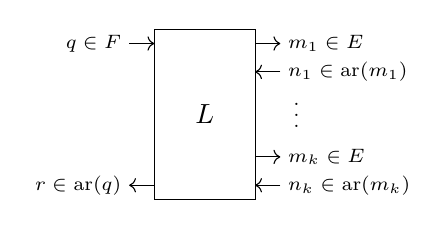
\begin{tikzpicture}[yscale=0.18,xscale=0.32]
      \draw (1,-1) rectangle (5,11) node[midway] {$L$};
      \scriptsize
      \draw[->] (0,10) node[left] {$q \in F$} -- (1,10);
        \draw[->] (5,10) -- (6,10) node[right] {$m_1 \in E$};
        \draw[->] (6,8) node[right] {$n_1 \in \kw{ar}(m_1)$} -- (5,8) ;
        \node[right] at (6,5.5) {$\:\vdots$};
        \draw[->] (5,2) -- (6,2) node[right] {$m_k \in E$};
        \draw[->] (6,0) node[right] {$n_k \in \kw{ar}(m_k)$} -- (5,0);
      \draw[->] (1,0) -- (0,0) node[left] {$r \in \kw{ar}(q)$};
    \end{tikzpicture}
  \end{column}
  \end{columns}

  \pause \vfill
  \begin{example}[Top-level and intermediate specifications]
    The strategies
    $\Gamma_\kw{hello},
     \Gamma_\kw{secret},
     \Gamma_\kw{decode} : \mathcal{S} \twoheadrightarrow \mathcal{P}$
    admit the behaviors:
    \begin{align*}
      \Gamma_\kw{hello} \: &\vDash \: \kw{run} \cdot
      \underline{\kw{write}_1[\texttt{"hello, world!\textbackslash{}n"}]} \cdot
      14 \cdot
      \underline{0}
    \\
    \uncover<3->{
      \Gamma_\kw{secret} \: &\vDash \: \kw{run} \cdot
      \underline{\kw{write}_1[\texttt{"uryyb, jbeyq!\textbackslash{}n"}]} \cdot
      14 \cdot
      \underline{0}
    }
    \\
    \uncover<4->{
      \Gamma_\kw{decode} \: &\vDash \: \kw{run} \cdot
      \underline{\kw{read}_0[100]} \cdot
      \texttt{"uryyb, jbeyq!\textbackslash{}n"} \cdot
      \underline{\kw{write}_1[\texttt{"hello, world!\textbackslash{}n"}]} \cdot
      14 \cdot
      \underline{0}
    }
    \end{align*}
  \end{example}

%  \pause \vfill
%  Strategies feature a simple ordering $\le$ (``is refined by'').
\end{frame}
%}}}

\begin{frame}{Layered Composition} %{{{
  The stragies $L_1 : F \twoheadrightarrow G$ and
  $L_2 : E \twoheadrightarrow F$ can be composed to obtain:
  \[
     L_1 \odot L_2 : E \twoheadrightarrow G
  \]
  \pause
  This is done by letting them interact over $F$
  in the following way:
  \[
    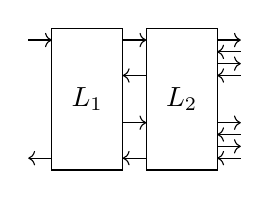
\begin{tikzpicture}[yscale=0.15,xscale=0.30]
      \draw (1,-1) rectangle (4,11) node[midway] {$L_1$};
      \draw (5,-1) rectangle (8,11) node[midway] {$L_2$};
      %\draw (5,-1) rectangle (8,4) node[midway] {$L_2$};
      \draw[->] (0,10) -- (1,10);
        \draw[->] (4,10) -- (5,10);
          \draw[->] (8,10) -- (9,10);
          \draw[->] (9,9) -- (8,9);
          \draw[->] (8,8) -- (9,8);
          \draw[->] (9,7) -- (8,7);
        \draw[->] (5,7) -- (4,7);
        \draw[->] (4,3) -- (5,3);
          \draw[->] (8,3) -- (9,3);
          \draw[->] (9,2) -- (8,2);
          \draw[->] (8,1) -- (9,1);
          \draw[->] (9,0) -- (8,0);
        \draw[->] (5,0) -- (4,0);
      \draw[->] (1,0) -- (0,0);
    \end{tikzpicture}
  \]

  \pause
  \begin{example}[Assembly linking]
    %To let $\kw{secret.s}$ call into $\kw{rot13.s}$ we can compute:
    %\[ \kw{Asm}(\kw{secret.s}) \odot \kw{Asm}(\kw{rot13.s}) \]
    A key ingredient in our example is
    the assembly linking theorem:
    \[ \ell \::\:
       \kw{Asm}(\kw{secret.s}) \odot \kw{Asm}(\kw{rot13.s}) \:\le\:
       \kw{Asm}(\kw{secret.s} + \kw{rot13.s}) \]
    The two strategies synchronize over $\kw{rot13()}$ calls,
    which become hidden internal calls.
  \end{example}
\end{frame}
%}}}

\begin{frame}{Flat Composition} %{{{
  Strategies can also be composed ``side by side'':
  \begin{itemize}
    \pause
    \item Effect signatures compose as $E_1 \oplus E_2$ (direct sum);
    \pause
    \item Strategies compose as $L_1 \oplus L_2 : E_1 \oplus E_2 \twoheadrightarrow F_1 \oplus F_2$.
  \end{itemize}

  \pause \vfill
  \begin{example}[Sequencing commands]
    Two commands $P, Q : \mathcal{S} \twoheadrightarrow \mathcal{P}$
    compose into
    $
      P \oplus Q \: : \:
        \mathcal{S} \oplus \mathcal{S} \: \twoheadrightarrow \:
        \mathcal{P} \oplus \mathcal{P}
    $.

    \pause \vspace{1ex}
    The simple component $\kw{seq} : \mathcal{P} \oplus \mathcal{P} \twoheadrightarrow \mathcal{P}$
    operates as:
    \[
      \kw{seq} \vDash \kw{run} \cdot \underline{\iota_1(\kw{run})} \cdot x
                               \cdot \underline{\iota_2(\kw{run})} \cdot y \cdot \underline{y}
    \]

    \pause
    The strategy
    $\Delta_\mathcal{S} : \mathcal{S} \twoheadrightarrow \mathcal{S} \oplus \mathcal{S}$
    can be used to combine their system calls:
    \[
      P \mathbin; Q \: := \:
        \kw{seq} \odot (P \oplus Q) \odot \Delta_\mathcal{S} \: : \:
        \mathcal{S} \twoheadrightarrow \mathcal{P}
    \]
  \end{example}

  \pause
  Together,
  $\odot$ and $\oplus$ form a
  symmetric monoidal category.
\end{frame}
%}}}

\begin{frame}[fragile]{Combining layered and flat composition} %{{{
  \begin{example}[Pipe operator]
    Given two commands $P, Q : \mathcal{F} \oplus \mathcal{F} \twoheadrightarrow \mathcal{P}$
    we can define:
    \[
      P \mathbin| Q \: := \:
        \kw{seq} \odot (P \oplus Q)
             \odot (\mathcal{F} \oplus (\Delta \odot \kw{fifo}) \oplus \mathcal{F})
      \quad \text{where} \quad
      \mathcal{S} \cong \mathcal{F} \oplus \mathcal{F}
    \]
    \[
      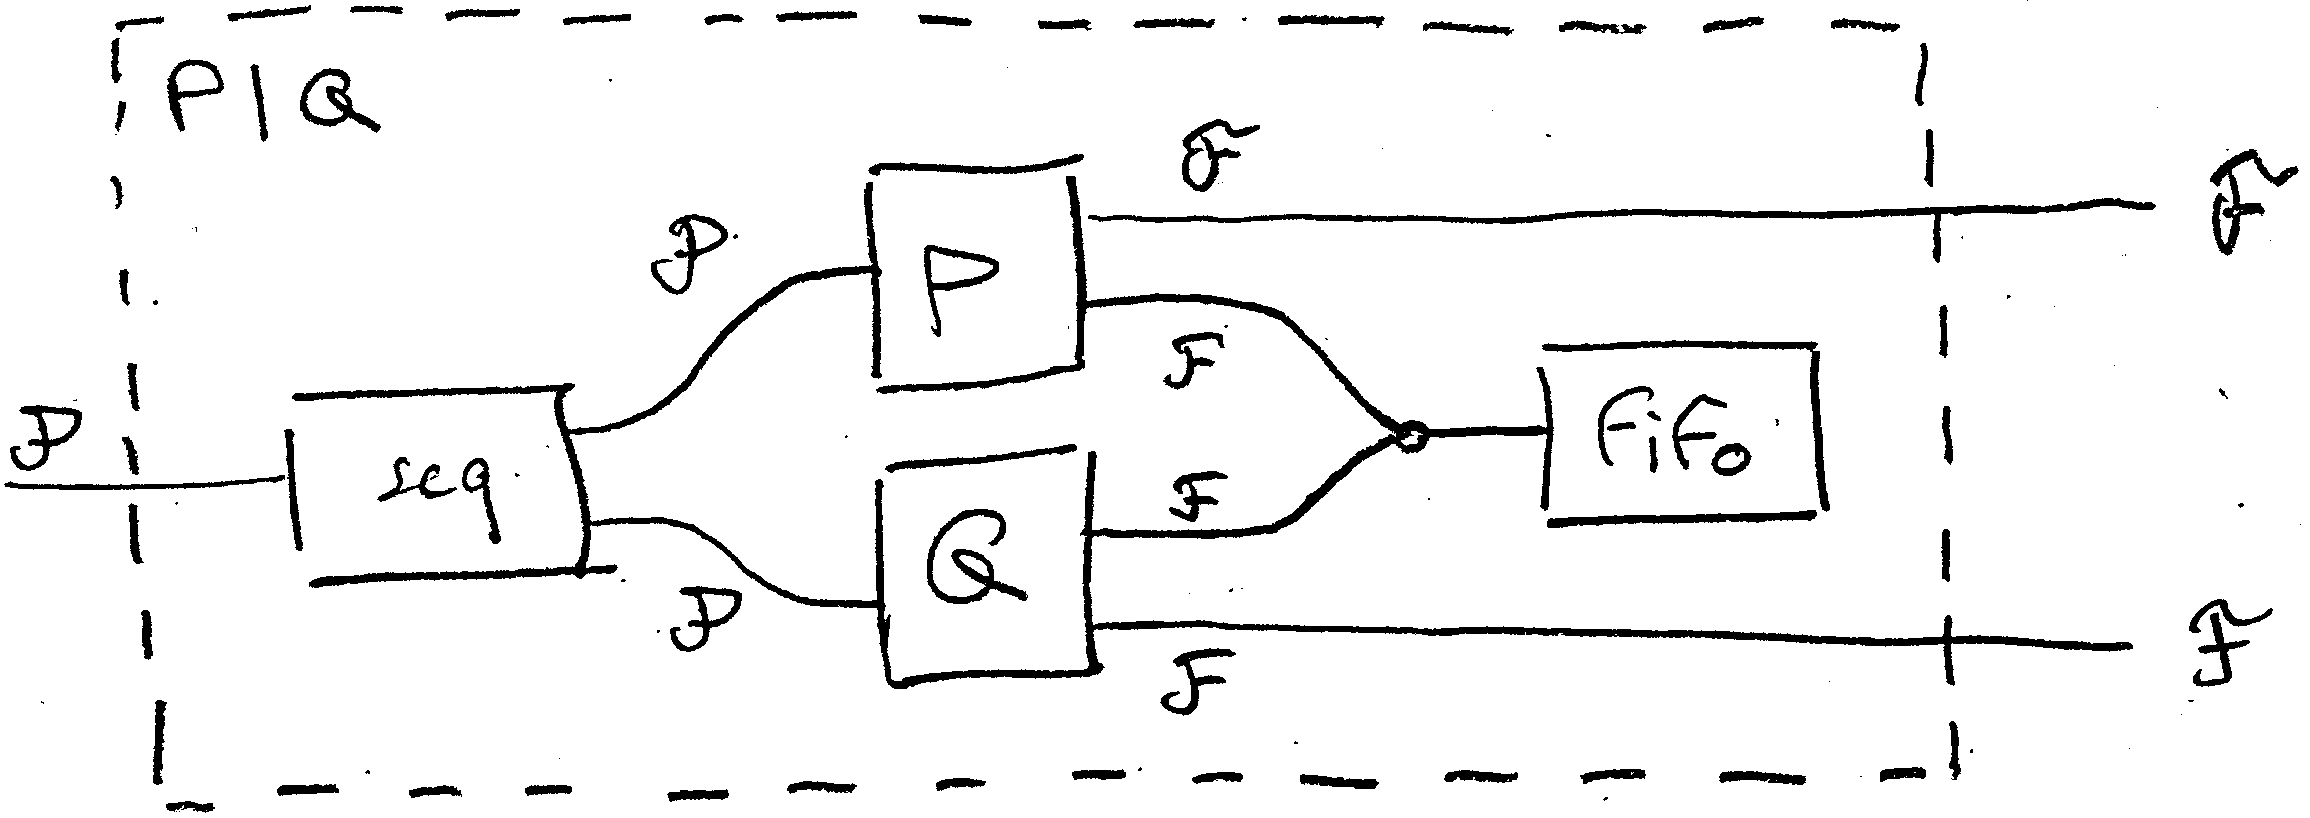
\includegraphics[scale=0.10]{pipe}
    \]
  This is how we define:
  \[
        M_\kw{encdec} \::=\:
        \kw{load}(\kw{secret.s} + \kw{rot13.s})
        \:\mathbin{\mathtt{|}}\:
        \kw{load}(\kw{decode.s} + \kw{rot13.s})
  \]
  \end{example}
\end{frame}
%}}}

\section{Vertical Composition and Refinement}

\begin{frame}[fragile]{Refinement Conventions and Refinement Squares} %{{{
Our framework comes with a simple notion of refinement:
\[
  \Gamma_\kw{hello} \le M_\kw{encdec}
  \qquad \qquad
  \begin{tikzcd}[sep=large]
    \mathcal{S} \ar[d,equal] \ar[r,"\Gamma_\kw{hello}", twoheadrightarrow] &
    \mathcal{P} \ar[d,equal] \\
    \mathcal{S} \ar[r, "M_\kw{encdec}"', twoheadrightarrow] & \mathcal{P}
  \end{tikzcd}
\]
\pause
To model abstraction relationships,
we introduce a notion of
\textbf{refinement conventions}:
\[
  \begin{tikzcd}[sep=huge]
    \mathcal{S} \ar[d,"\kw{runtime}_*"', leftrightarrow]
      \ar[r, "\Gamma_\kw{decode}", twoheadrightarrow] &
    \mathcal{P} \ar[d,"\kw{entry}^*", leftrightarrow] \\
    \mathcal{C} \mathbin@ \kw{mem} \ar[r, "\kw{Clight}(\kw{decode.c})"', twoheadrightarrow] &
    \mathcal{C} \mathbin@ \kw{mem}
  \end{tikzcd}
  \qquad \pause
  \begin{tikzcd}[sep=huge]
    \mathcal{C} \mathbin@ \kw{mem} \ar[d, "\mathbb{C}"', leftrightarrow]
      \ar[r, "\kw{Clight}(\kw{decode.c})", twoheadrightarrow] &
    \mathcal{C} \mathbin@ \kw{mem} \ar[d, "\mathbb{C}", leftrightarrow] \\
    \mathcal{A} \mathbin@ \kw{mem} \ar[r, "\kw{Asm}(\kw{decode.s})"', twoheadrightarrow] &
    \mathcal{A} \mathbin@ \kw{mem}
  \end{tikzcd}
\]
\end{frame}
%}}}

\begin{frame}[fragile]{Vertical Composition} %{{{
  \begin{columns}
    \begin{column}{0.7\textwidth}
      As expected, refinement $\le$ is transitive:
      \[
        \begin{prooftree}
          \hypo{\only<2->{\phi : } L_1
            \le\only<5->{_{\mathbf{R} \twoheadrightarrow \mathbf{S} }}
            L_2}
          \hypo{\only<2->{\psi : } L_2
            \le\only<5->{_{\mathbf{R'} \twoheadrightarrow \mathbf{S'} }} L_3}
          \infer2{\only<3->{\phi \vcomp \psi : }
            L_1
              \le\only<6->{_{\mathbf{R} \vcomp \mathbf{R'} \twoheadrightarrow
                \mathbf{S} \vcomp \mathbf{S'} }}
            L_3}
        \end{prooftree}
      \]

      \uncover<4->{%
        The \emph{vertical composition} principle $\vcomp$ \\
        applies to refinement conventions as well.
      }

      \vspace{1em}
      \uncover<7->{%
        \begin{example}[Correctness and compilation]
          We can combine C code verification
          and compiler correctness properties
          to relate spec and assembly code directly:
          \[
            \begin{prooftree}
              \hypo{
                \Gamma_\kw{decode}
                \le_{\mathbf{R} \twoheadrightarrow \mathbf{S}}
                \kw{Clight}(\kw{decode.c})
                \le_{\mathbb{C} \twoheadrightarrow \mathbb{C}}
                \kw{Asm}(\kw{decode.s})}
              \infer1{
                \Gamma_\kw{decode}
                \le_{\mathbf{R} \vcomp \mathbb{C} \twoheadrightarrow
                     \mathbf{S} \vcomp \mathbb{C}}
                \kw{Asm}(\kw{decode.s})}
            \end{prooftree}
          \]
        \end{example}
      }
    \end{column}
    \begin{column}{0.25\textwidth}
      \[
        \begin{tikzcd}[sep=small]
          E\only<5->{_1} \ar[rr, "L_1", twoheadrightarrow]
              \only<-2>{\ar[dd, equal]}
              \only<3-4>{\ar[dddd,equal]}
              \only<5>{\ar[dd, "\mathbf{R}"', leftrightarrow]}
              \only<6->{\ar[dddd, "\mathbf{R} \vcomp \mathbf{R}'"', leftrightarrow]}
              &&
          F\only<5->{_1}
              \only<-2>{\ar[dd, equal]}
              \only<3-4>{\ar[dddd,equal]}
              \only<5>{\ar[dd, "\mathbf{S}", leftrightarrow]}
              \only<6->{\ar[dddd, "\mathbf{S} \vcomp \mathbf{S}'", leftrightarrow]}
          \\
          & \only<1,3-4,6->{\color{white}} \phi &
          \\
          \only<-2,5>{
          E\only<5->{_2} \ar[rr, "L_2", twoheadrightarrow]
            \only<-4>{\ar[dd, equal]}
            \only<5->{\ar[dd, "\mathbf{R}'"', leftrightarrow]}
          }
          &
          \only<-2,5>{\color{white}}
          \!\!\!\! \phi \vcomp \psi \!\!\!\!
          &
          \only<-2,5>{
          F\only<5->{_2}
            \only<-4>{\ar[dd, equal]}
            \only<3->{\ar[dd, "\mathbf{S}'", leftrightarrow]}
          }
          \\
          & \only<1,3-4,6->{\color{white}} \psi &
          \\
          E\only<5->{_3} \ar[rr, "L_3", twoheadrightarrow]
              &&
          F\only<5->{_3}
        \end{tikzcd}
      \]
    \end{column}
  \end{columns}
\end{frame}
%}}}

\begin{frame}<3-4,6->[fragile]{Layered Composition of Refinement Squares} %{{{
  Refinement is compatible with composition
  in the expected way:
  \[
    \begin{prooftree}
      \hypo{\only<3->{\phi:} L_1
         \le\only<6->{_{\mathbf{S} \twoheadrightarrow \mathbf{T} }} L_1'}
      \hypo{\only<3->{\psi:} L_2
         \le\only<6->{_{\mathbf{R} \twoheadrightarrow \mathbf{S} }} L_2'}
      \infer2{\only<3->{\phi \odot \psi \: : \: }
	L_1 \odot L_2 \:
        \le\only<6->{_{\mathbf{R} \twoheadrightarrow \mathbf{T} }}
        \: L_1' \odot L_2'}
    \end{prooftree}
  \]

  \pause
  This can be depicted as:

  \[
    \rule[-4em]{0pt}{8em}
    \begin{tikzcd}[sep=small]
       E \only<-3,5-6>{\ar[rr,"L_2",twoheadrightarrow]}
         \only<4,7->{\ar[rrrr,"L_1 \odot L_2",twoheadrightarrow]}
         \only<-5>{\ar[dd,equal]}
         \only<6->{\ar[dd,leftrightarrow,"\mathbf{R}"']}
       &&
       \only<-3,5-6>{%
       F \ar[rr,"L_1",twoheadrightarrow]
         \only<-5>{\ar[dd,equal]}
         \only<6->{\ar[dd,leftrightarrow,"\mathbf{S}"]}
       }%
       &&
       G \only<-5>{\ar[dd,equal]}
         \only<6->{\ar[dd,leftrightarrow,"\mathbf{T}"]}
       \\
       & \only<-2>{\le} \only<3,5-6>{\phi} &
         \only<4,7->{\phi \odot \psi} &
         \only<-2>{\le} \only<3,5-6>{\psi} &
       \\
       E\only<6->{'}
          \only<-3,5-6>{\ar[rr,"L_2'"',twoheadrightarrow]}
          \only<4,7->{\ar[rrrr, "L_1' \odot L_2'"', twoheadrightarrow]}
       &&
       \only<-3,5-6>{
         F\only<6->{'} \ar[rr,"L_1'"',twoheadrightarrow]
       }
       &&
       G\only<6->{'} \\
    \end{tikzcd}
  \]

  \uncover<8>{Similar rules apply for flat composition.}
\end{frame}
%}}}

%\begin{frame}[fragile]{Flat Composition of Refinement Squares} %{{{
%  Flat composition $\oplus$ acts
%  on refinement conventions and refinement squares as well:
%  \pause
%  \[
%    \begin{tikzcd}[sep=tiny]
%      E_1 \ar[rrrrrr, twoheadrightarrow, "L_1"]
%          \ar[dddddd, leftrightarrow, "\mathbf{R_1}"']
%          \ar[rd, dotted, dash] & & &&&&
%      F_1 \ar[dddddd, leftrightarrow, "\mathbf{S_1}"]
%          \ar[rd, dotted, dash]  & & \\
%      & \oplus \ar[rd, dotted, dash] & &&&&
%      & \oplus \ar[rd, dotted, dash] & \\
%      & & E_2 \ar[rrrrrr, twoheadrightarrow, "L_2"]
%              \ar[dddddd, leftrightarrow, "\mathbf{R}_2"'] &&&&
%      & & F_2 \ar[dddddd, leftrightarrow, "\mathbf{S}_2"] \\
%      \\ &&&& \color{white} \Big| XX \\ \\
%      E_1' \ar[rrrrrr, twoheadrightarrow, "L_1'"']
%           \ar[rd, dotted, dash] & & &&&&
%      F_1' \ar[rd, dotted, dash] & & \\
%      & \oplus \ar[rd, dotted, dash] & &&&&
%      & \oplus \ar[rd, dotted, dash] & \\
%      & & E_2' \ar[rrrrrr, twoheadrightarrow, "L_2'"'] &&&&
%      & & F_2'
%    \end{tikzcd}
%    \qquad
%    \begin{array}{c}
%    \begin{prooftree}
%      \hypo{L_1 : E_1 \twoheadrightarrow F_1}
%      \hypo{L_2 : E_2 \twoheadrightarrow F_2}
%      \infer2{
%        L_1 \oplus L_2 : E_1 \oplus E_2 \twoheadrightarrow F_1 \oplus F_2}
%    \end{prooftree}
%    \\[2em] \pause
%    \begin{prooftree}
%      \hypo{\mathbf{R} : E_1 \leftrightarrow F_1}
%      \hypo{\mathbf{S} : E_2 \leftrightarrow F_2}
%      \infer2{
%        \mathbf{R} \oplus \mathbf{S} : E_1 \oplus E_2 \leftrightarrow F_1 \oplus F_2
%      }
%    \end{prooftree}
%    \\[2em] \pause
%    \begin{prooftree}
%      \hypo{\phi: L_1 \le_{\mathbf{R}_1 \twoheadrightarrow \mathbf{S}_1} L_1'}
%      \hypo{\psi: L_2 \le_{\mathbf{R}_2 \twoheadrightarrow \mathbf{S}_2} L_2'}
%      \infer2{\phi \oplus \psi :
%	L_1 \oplus L_2
%        \le_{\mathbf{R}_1 \oplus \mathbf{R}_2 \twoheadrightarrow
%             \mathbf{S}_1 \oplus \mathbf{S}_2}
%	L_1' \oplus L_2'}
%    \end{prooftree}
%    \end{array}
%  \]
%\end{frame}
%%}}}

\section{Spatial Composition}

%\begin{frame}{Motivation} %{{{
%Our history-based strategy and refinement convention models \\
%support hidden state, but this is not always what we want.
%
%\vfill \pause
%Ideally, we would like our refinement algebra to support state which is:
%\begin{itemize}
%  \item Visible locally, but hidden when we work on the next scale;
%  \item Abstract at a high level of abstraction, more concrete as we implement;
%  \item Hidden in specifications, but realized using low-level explicit memory.
%\end{itemize}
%
%\vfill \pause
%Do deal with state in a flexible manner,
%we introduce a \textbf{spatial composition} operator $\mathbin@$, \\
%then leverage our refinement algebra to introduce
%useful state management primitives.
%\end{frame}
%}}}

\begin{frame}{Spatial Composition} %{{{
  Our last composition principle is \emph{spatial composition} $\mathbin@$,
  which acts on:
  \pause
  \begin{itemize}
    \item Effect signatures
    \[
      E \mathbin@ U := \{ m @ u \mathbin: N \times U \mid
            m\mathbin:N \in E, \, u \in U \}
    \]

    \pause
    \item Strategies (and \emph{stateful lenses})
      \[
        \begin{prooftree}
          \hypo{L : E \twoheadrightarrow F}
          \hypo{f : U \leftrightarrows V}
          \infer2{L \mathbin@ f : E \mathbin@ U \twoheadrightarrow
                                  F \mathbin@ V}
        \end{prooftree}
      \]

    \pause
    \item Refinement conventions (where $U$ is interpreted as
         $\{ u : U \mid u \in U \}$)
      \[
        \begin{prooftree}
          \hypo{\mathbf{R} : E \leftrightarrow F}
          \hypo{\mathbf{S} : 
            U
            \leftrightarrow
            V}
          \infer2{\mathbf{R} \mathbin@ \mathbf{S} :
                    E \mathbin@ U \leftrightarrow
                                  F \mathbin@ V}
        \end{prooftree}
      \]

    \pause
    \item Refinement squares
  \end{itemize}
\end{frame}
%}}}

\begin{frame}{Encapsulating State} %{{{
  \begin{example}[Invoking $\kw{main}$]
    A component
    $\kw{entry} : \mathcal{C} \mathbin@ \kw{mem} \twoheadrightarrow \mathcal{P}$
    can be constructed as follows:
    \pause
    \begin{itemize}
      \item Call the main function using a component
      $L_\kw{invoke} : \mathcal{C} \twoheadrightarrow \mathcal{P}$
      \[ L_\kw{invoke} \: \vDash \:
         \kw{run} \cdot \underline{\kw{main}(\epsilon)} \cdot
         \kw{Vint}(n) \cdot n \]

      \pause
      \item Hide the memory state using a component
        $[m_0\rangle : \kw{mem} \leftrightarrows \mathbbm1$
      \[ \kw{entry} \: := \:
         L_\kw{invoke} \mathbin@ [m_0\rangle \: : \:
         \mathcal{C} \mathbin@ \kw{mem} \: \twoheadrightarrow \:
         \mathcal{P} \mathbin@ \mathbbm1 \pause \: \cong \:
         \mathcal{P} \]
    \end{itemize}
  \end{example}

  \pause
  The \textbf{encapsulation primitive}
  $[u_0 \rangle : U \leftrightarrows \mathbbm1$
  can be defined for any $u_0 \in U$.
  \\
  \pause
  Refinement squares capture \emph{simulation} arguments
  for representation independence.
\end{frame}
%}}}

%\begin{frame}{Manipulating state components} %{{{
%To act on state components,
%we use a kind of \textbf{stateful lenses}
%$f : U \lensarrow V$ \\
%which can be spatially composed with strategies:
%\[
%  \begin{prooftree}
%    \hypo{L : E \twoheadrightarrow F}
%    \hypo{f : U \lensarrow V}
%    \infer2{L \mathbin@ f : E \mathbin@ U \twoheadrightarrow F \mathbin@ V}
%  \end{prooftree}
%\]
%
%\pause
%Similarly, relations between sets can be promoted to \\
%and composed with refinement conventions: \\
%\[
%  \begin{prooftree}
%    \hypo{\mathbf{R} : E \leftrightarrow F}
%    \hypo{S \subseteq U \times V}
%    \infer2{\mathbf{R} \mathbin@ S : E \mathbin@ U \twoheadrightarrow F \mathbin@ V}
%  \end{prooftree}
%\]
%
%\pause
%We also define refinement squares between lenses and they compose as expected.
%\end{frame}
%}}}

\begin{frame}[fragile]{Memory Separation} %{{{
  A separation algebra $\bullet$ defines a relation
  $\mathsf{Y} \subseteq (\kw{mem} \times \kw{mem}) \times \kw{mem}$
  where
  \[
    (m_1, m_2) \mathrel{\mathsf{Y}} m \:\: :\Leftrightarrow \:\:
    m_1 \bullet m_2 = m
  \]
  The relation $\mathsf{Y}$ can then be promoted
  to a refinement convention component.

  \pause \vfill
  This allows us to formulate refinement-based \textbf{frame properties};
  for example:
%  \[
%    \mathsf{FP}(p) \: : \:
%    \kw{Clight}(p) \mathbin@ \kw{mem}
%    \:
%    \le_{\mathcal{C} \mathbin@ \mathsf{Y} \twoheadrightarrow
%         \mathcal{C} \mathbin@ \mathsf{Y}}
%    \:
%    \kw{Clight}(p)
%  \]
  \[
    \begin{tikzcd}[row sep=small]
      \mathcal{C} \mathbin@ \kw{mem} \mathbin@ \kw{mem}
        \ar[rr, "\kw{Clight}(p) \mathbin@ \kw{mem}"]
        \ar[dd, "\mathcal{C} \mathbin@ \mathsf{Y}"', leftrightarrow] &&
      \mathcal{C} \mathbin@ \kw{mem} \mathbin@ \kw{mem}
        \ar[dd, "\mathcal{C} \mathbin@ \mathsf{Y}", leftrightarrow]
      \\
      & \mathsf{FP}(p) &
      \\
      \mathcal{C} \mathbin@ \kw{mem}
        \ar[rr, "\kw{Clight}(p)"'] &&
      \mathcal{C} \mathbin@ \kw{mem}
    \end{tikzcd}
  \]
\end{frame}
%}}}

\section{Conclusion}

\begin{frame}{Conclusion} %{{{
  By combining these ingredients,
  we were able to apply the framework in various ways:
  \begin{itemize}
    \pause
    \item Incorporate \textbf{CompCertO} semantics and correctness results
    \pause
    \item Define a new language ClightP with \textbf{private variables}
    \pause
    \item Construct a theory of \textbf{certified abstraction layers}
    \pause
    \item Model the example from the introduction
  \end{itemize}

  \pause
  I hope to have convinced you that
  \begin{quote}
    Such frameworks can be a
    \textbf{coarse-grained glue} for heterogeneous verification, \\
    and become the basis for
    \textbf{reusable certified software components}.
  \end{quote}

  \pause
  To pursue this further we would like to:
  \begin{itemize}
    \item Add \textbf{concurrency} to the model
    \pause
    \item Make more explicit connections to \textbf{higher category theory}
  \end{itemize}
\end{frame}
%}}}

\begin{frame} %{{{
  \Large \centering Thank you!
\end{frame}
%}}}

\appendix

\begin{frame}[fragile]{Representation Independence} %{{{
  When the initial states $u_0 \in U$ and $v_0 \in V$
  are related by $R \subseteq U \times V$,
  the refinement
  \[
    \begin{prooftree}
      \hypo{\phi_0 : u_0 \mathrel{R} v_0}
      \infer1{[\phi_0\rangle :
         [u_0\rangle \le_{R \twoheadrightarrow \mathbbm{1}}
         [v_0\rangle}
    \end{prooftree}
    \qquad \qquad
    \begin{tikzcd}[sep=tiny]
      U \ar[dd, "R"', leftrightarrow] \ar[rr, "{[u_0\rangle}"] &&
      \mathbbm{1} \ar[dd, equal] \\
      & {[ \phi_0 \rangle} & \\
      V \ar[rr, "{[v_0\rangle}"'] & & \mathbbm{1}
    \end{tikzcd}
  \]
  captures a form of \textbf{representation independence} property.

  \vfill \pause
  \begin{example}[continue previous example]
  \end{example}
\end{frame}
%}}}

\end{document}
